\chapter{Visible Surface}
Es geht darum, unsichtbare Flächen nicht darstellen zu lassen - sonst sieht es ja komisch aus.

\section{Backface Culling}
Wenn die Objekte geschlossen sind, dann kann einfach der Normalenvektor der Fläche betrachtet werden - denn wenn ein Vektor wegzeigt muss diese Fläche liegt dann ja auf der Rückseite und muss logischerweise nicht gezeichnet werden.

\section{Tiefensortierung}
Sortiere die Polygone und zeichne sie dann von hinten nach vorne, sodass die zuletzt gezeichneten Polygone die anderen überdecken. Wird auch als \textit{Maleralgorithmus} bezeichnet.
\subsection{Vorteile}
\begin{enumerate}
	\item Auch für transparente Objekte möglich
	\item Einfach für Spezialfälle
\end{enumerate}
\subsection{Nachteile}
\begin{enumerate}
	\item Ineffizient für viele Objekte \(O(n^2)\)
	\item Wird nicht direkt Hardware unterstützt
	\item Nicht für jedes Objekt direkt möglich - unpassende Objekte  müssen z.B. noch weiter zerschnitten werden
\end{enumerate}
\subsection{Details}
Im Detail sieht das dann so aus:
Von jedem Polygon wird der Punkt genommen, der am nächsten zur Kamera ist. Anhand dieser Entfernen werden die Polygone zuerst einmal grob sortiert. Wenn jetzt sich irgendwo Polygone überschneiden, also z.B. Polygon A ist zwischen 2 und 10 von der Kamera entfernt und Polygon B zwischen 8 und 11, dann wird noch weiteres gemacht.

Polygon A ist zur Zeit jetzt ja näher bei der Kamera. Falls nun irgend eine folgende Bedingung zutrifft, werden sie nicht vertauscht, ansonsten schon.

\begin{enumerate}
	\item \textbf{Überlagern sich die x-Ausdehnungen nicht?} \\
	Auf gut Deutsch: Sind die Objekte vollständig nebeneinander?
	\item \textbf{Überlagern sich die y-Ausdehnungen nicht?} \\
	Sind die Objekte vollständig hintereinander? Abbildung \ref{fig:ausdehnungen} zeigt ein Beispiel, wo die Objekte vollständig nebeneinander sind, aber nicht vollständig hintereinander.
	\begin{figure}[!ht]
		\centering
		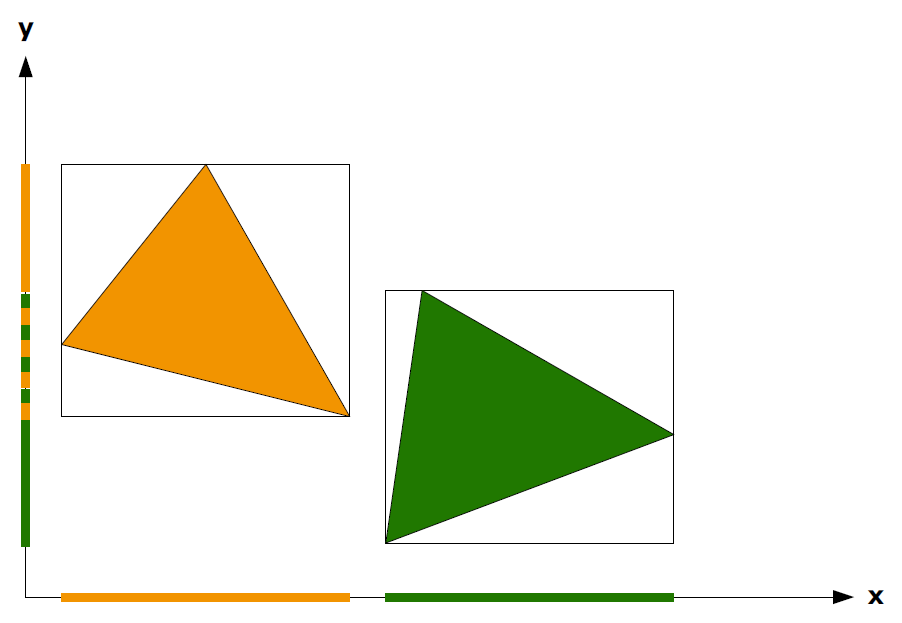
\includegraphics[width=0.5\linewidth]{fig/ausdehnungen}
		\caption{Beispiel Ausdehnung von 2 Objekten}
		\label{fig:ausdehnungen}
	\end{figure}
	\item \textbf{Liegt das hintere Objekt ganz auf der vom Betrachter abgewandeten Seite vom vorderen Objekt?} \\
	Kein Plan was das bedeuteten soll.
	\begin{figure}[!ht]
		\centering
		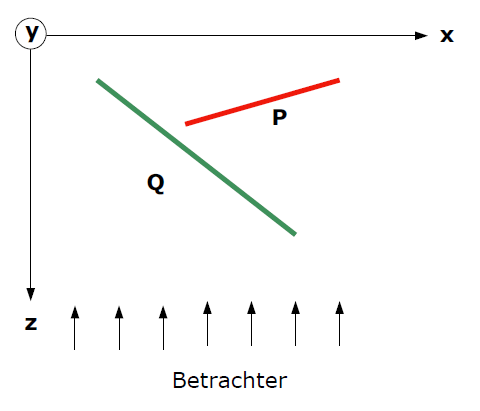
\includegraphics[width=0.5\linewidth]{fig/tiefensortierung_3}
		\caption{Ein Beispiel dazu}
		\label{fig:tiefensortierung_3}
	\end{figure}
	\item \textbf{Liegt das vordere Objekt komplett auf der Betrachterseite vom vorderen Objekt?}\\
	\begin{figure}[!ht]
		\centering
		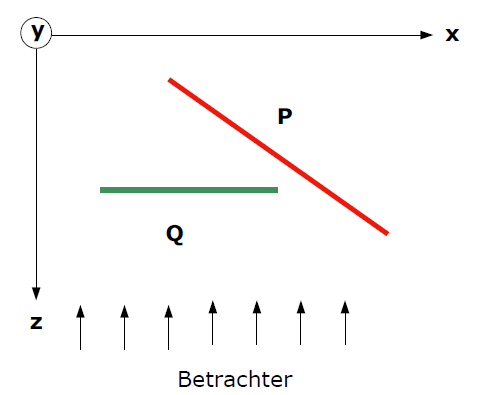
\includegraphics[width=0.5\linewidth]{fig/tiefensortierung_4}
		\caption{Ein Beispiel dazu}
		\label{fig:tiefensortierung_4}
	\end{figure}
	\item \textbf{Überlappen sich die Polygone nicht auf der Projektion in die xy Ebene?}\\
	\begin{figure}[!ht]
		\centering
		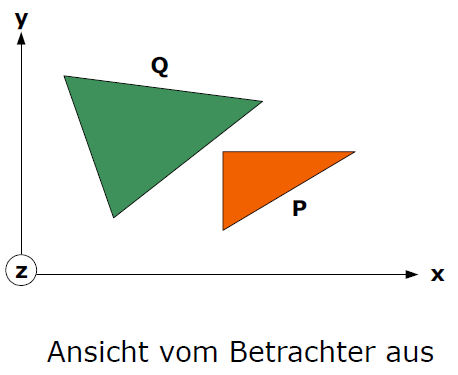
\includegraphics[width=0.5\linewidth]{fig/tiefensortierung_5}
		\caption{Ein Beispiel dazu}
		\label{fig:tiefensortierung_5}
	\end{figure}
	Nehmen wir an, die beiden Objekte sind die zwei Dreiecke - wenn wir jetzt stur von vorne auf diese Objekte schauen, sind diese ja 2-Dimensional. Wenn sich diese nicht schneiden, wie im Beispiel in Abbildung \ref{fig:tiefensortierung_5}, dann ist diese Bedingung erfüllt.
	
\end{enumerate}
\section{Z Buffer}
Auf Grund der Nachteile vom Tiefensortieren hat man einen ganz einfachen Algorithmus entwickelt. Dieser zeichnet alle Polygone, berechnet also die R, G und B Werte und zusätzlich noch die Entfernung zur Kamera - der Z Wert. Beim Zeichnen der Pixel wird dann einfach geprüft, ob der aktuelle Pixel näher ist.
\subsection{Vorteile}
\begin{enumerate}
	\item Hardwareunterstützt
	\item Polygone können in beligiger Reihenfolge gezeichnet werden
	\item Zeitkomplexität ist O(n), aber häufig sogar konstant ab einer gewissen Anzahl Polygone.
\end{enumerate}
\subsection{Nachteile}
\begin{enumerate}
	\item Rundungsprobleme
	\item Was ist, wenn zwei Pixel denselben z Wert haben? (Dann gibts Artefakte vom überlappen)
	\item (grosser Speicherbedarf - heute nicht mehr soo problematisch)
\end{enumerate}
\subsection{Berechnung von z}
Z lässt sich aus der Ebenengleichung berechnen
\begin{displaymath}
z = \frac{-D-Ax-By}{C}
\end{displaymath}
oder inkrementell entlang einer Scanlinie
\begin{displaymath}
z_{neu} = \frac{-D-A(x_{alt}+1)-By}{C}=z_{alt}-\frac{A}{C}
\end{displaymath}


\section{Warnock Algorithmus}
Hier wird der Bildbereich angeschaut und entschieden, ob er \textit{einfach} zu zeichnen ist. Ist er das nicht, wird er in 4 Unterbereiche unterteilt, für welche dann wieder einzeln entschieden wird, ob sie \textit{einfach} sind. Das ist dementsprechend rekursiv.
\subsection{Einfache Bereiche}
Ein Bereich ist einfach, falls...
\begin{enumerate}
	\item ... er kein oder nur 1 Polygon enthält.
	\item ... nur ein Polygon beinhaltet, das am nächsten ist und den Bereich auch vollständig füllt.
	\item ... er nur 1 Pixel gross ist.
\end{enumerate}
\begin{figure}[!ht]
	\centering
	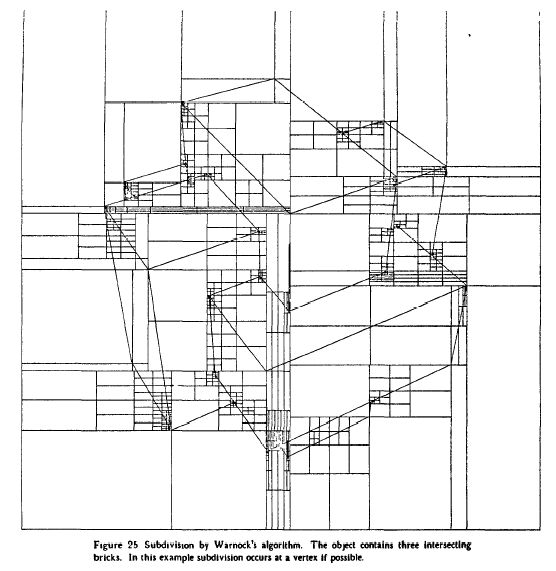
\includegraphics[width=0.5\linewidth]{fig/warnock}
	\caption{Ein Beispiel zu Warnock}
	\label{fig:warnock}
\end{figure}
\section{Various}
Ein Ausdehnungsbereich ist ein möglichst kleines Rechteck (Bounding Box), welches das Objekt vollständig enthält. Wenn sich solche Ausdehnungsbereiche nicht schneiden, so schneiden sich logischerweise auch die Objekte nicht.\\
Objektraum = alle Objekte\\
Bildraum = alle Pixel